\section{Problem Set 7} \label{sec:7}

\subsection{Recap of Relative Orbital Work}
Over the past two problem sets, we were able to successfully implement two methods of relative orbit control. The first method was using a naive least squares formulation for impulsive control and station keeping. The second method was using a Lyapunov-value function based optimal control method for continuous control, also used for both station keeping and orbital reconfiguration maneuvers. The main takeaways so far are:
\begin{itemize}
    \item The naive-least squares method is sub-optimal, using much more fuel than the lower bound. The benefit of this is that the maneuvers can be completed in a short time-frame. 
    \item Without a thrust constraint and proper tuning of the hyper-parameters, the continuous control uses significantly more $\Delta v$ than the impulsive control methods. The continuous control also requires significantly larger time windows to reach its target.
\end{itemize}
Based on these prior lessons, the next steps would be to use impulsive control, but use a closed-form solution based on reachable set theory that requires less $\Delta v$ than the current naive least-squares implementation. We do not have a requirement on our system for the thrusters we can use, so using continuous control with sub-optimal results and hyperparameter tuning does not make sense. The closed-form control method will be implemented along with the navigation work in Problem Set 8.

The team will also test run a method based on sequential convex optimization, in hopes that that provides a global minimum continuous control policy in terms of fuel usage. If this performs comparably to the impulsive control in terms of thrust (i.e. accounting for the continuous control having a much higher $I_{sp}$), then we may finalize with using SCP-based control.

\subsection{Initial Navigation System Design}

\subsubsection{Choice of State Representation} \label{sec:nav_state_rep}
We will be using an Extended Kalman Filter (EKF) for our navigation system. Within the EKF, we will use a mixed state representation of absolute and relative orbit elements of the chief and deputies. Specifically, we will estimate the absolute orbit elements of the chief and the relative orbit elements of the deputy. The resulting state vector is:

\begin{equation}
\begin{bmatrix}
\boldsymbol{\alpha}_1 \\
\hline
\delta \boldsymbol{\alpha}_2 \\
\hline
\delta \boldsymbol{\alpha}_3
\end{bmatrix}
=
\begin{bmatrix}
a_1 \\
e_{x,1} \\
e_{y,1} \\
i_1 \\
\Omega_1 \\
u_1 \\
\hline
\delta a_2 \\
\delta \lambda_2 \\
\delta e_{x,2} \\
\delta e_{y,2} \\
\delta i_{x,2} \\
\delta i_{y,2} \\
\hline
\delta a_3 \\
\delta \lambda_3 \\
\delta e_{x,3} \\
\delta e_{y,3} \\
\delta i_{x,3} \\
\delta i_{y,3}
\end{bmatrix}
\end{equation}

This state representation was chosen because we are not assuming perfect knowledge of the absolute chief state, so we must estimate it. This estimated absolute chief state then informs our estimation of the relative states of the deputies, which are inherently the focus of our docking and servicing mission. Orbit elements in general were chosen because they give more immediately intuitive understandings of the relative state and change much less rapidly then Cartesian position and velocity do. This makes it easier for our filter to accurate estimate the state since the magnitude of propagation steps is smaller. 

\subsubsection{Dynamics Model for State Prediction}
For predicting the state within the filter, two different dynamics models will be used. For predicting the absolute chief orbit elements, the nonlinear Gauss Variational Equations (GVEs) will be numerically integrated. This approach is outlined in Section \ref{sec:osc_mean_J2}. For predicting the relative orbit elements of the deputies, the ROEs will be propagated via numerical integration of the following expression from Koenig \cite{koenig2017new}:

\begin{equation}
\delta \dot{\boldsymbol{\alpha}_{\text{qns}'}} = 
\kappa_d
\begin{pmatrix}
0 \\
\eta_d(3\cos^2 i_d - 1) + (5\cos^2 i_d - 1) - 2\cos i_d \cos i_c \\
- e_d \sin(\omega_d - \omega_c)(5\cos^2 i_d - 1) \\
e_d \cos(\omega_d - \omega_c)(5\cos^2 i_d - 1) \\
0 \\
-2\cos i_d \sin i_c
\end{pmatrix}
-
\kappa_c
\begin{pmatrix}
0 \\
(1 + \eta_c)(3\cos^2 i_c - 1) \\
- e_d \sin(\omega_d - \omega_c)(5\cos^2 i_c - 1) \\
e_d \cos(\omega_d - \omega_c)(5\cos^2 i_c - 1) \\
0 \\
-2\cos i_c \sin i_c \\
\end{pmatrix}
\label{eq:ROE_nonlinear}
\end{equation}

where:
\begin{align*}
\eta_d &= \sqrt{1 - e_d^2} \\
\eta_c &= \sqrt{1 - e_c^2} \\
\\
\kappa_d &= \frac{3 J_2 R_E^2 \sqrt{\mu}}{4 a_d^{7/2} \eta_d^4} \\
\kappa_c &= \frac{3 J_2 R_E^2 \sqrt{\mu}}{4 a_c^{7/2} \eta_c^4}
\end{align*}

This expression is the non-linear time derivative of the modified ROE, and thus can be used for propagation. Note that this expression uses the modified ROEs to obtain a more sparse plant matrix. The modified ROEs are defined as:
\begin{equation}
\delta \boldsymbol{\alpha}_{\text{qns}'} = \mathbf{J}_{\text{qns}}(\alpha_c) \, \delta \boldsymbol{\alpha}_{\text{qns}}
\end{equation}

where:
\begin{equation}
\mathbf{J}_{\text{qns}}(\alpha_c) =
\begin{bmatrix}
\mathbf{I}_{2 \times 2} & \mathbf{0}_{2 \times 2} & \mathbf{0}_{2 \times 2} \\
\mathbf{0}_{2 \times 2} & 
\begin{bmatrix}
\cos \omega & \sin \omega \\
-\sin \omega & \cos \omega
\end{bmatrix}
& \mathbf{0}_{2 \times 2} \\
\mathbf{0}_{2 \times 2} & \mathbf{0}_{2 \times 2} & \mathbf{I}_{2 \times 2}
\end{bmatrix}
\end{equation}

and where the modified ROE are defined as:
\begin{equation}
\delta \boldsymbol{\alpha}_{\text{qns}'} =
\begin{pmatrix}
\delta a \\
\delta \lambda \\
\delta e_{x'} \\
\delta e_{y'} \\
\delta i_x \\
\delta i_y
\end{pmatrix}
=
\begin{pmatrix}
\frac{a_d - a_c}{a_c} \\
(M_d - M_c) + (\omega_d - \omega_c) + (\Omega_d - \Omega_c) \cos i_c \\
e_d \cos(\omega_d - \omega_c) - e_c \\
e_d \sin(\omega_d - \omega_c) \\
i_d - i_c \\
(\Omega_d - \Omega_c) \sin i_c
\end{pmatrix}
\end{equation}

Using these expressions, we can propagate ROE for each discrete time step, transforming from quasi-nonsingular ROE to modified quasi-non-singular ROE appropriately. This propagation only takes into account Keplerian and J2 effects and does not include control inputs. 

To propagate with control inputs, the control input matrix defined by Chernick is used \cite{chernick2021optimal}:
\begin{equation}
\Delta \delta \boldsymbol{\alpha}_k = \boldsymbol{\Gamma}_k \delta \mathbf{v}_k = 
\frac{1}{n a}
\begin{bmatrix}
0 & 2 & 0 \\
-2 & 0 & 0 \\
\sin(u_k) & 2 \cos(u_k) & 0 \\
-\cos(u_k) & 2 \sin(u_k) & 0 \\
0 & 0 & \cos(u_k) \\
0 & 0 & \sin(u_k)
\end{bmatrix}
\begin{bmatrix}
\delta v_R \\
\delta v_T \\
\delta v_N
\end{bmatrix}
\label{eq:control_input_matrix}
\end{equation}

At every discrete time step, the filter prediction step checks to see if there is a control input. If there is an applied delta-v then the above expression is used to find the instantaneous change in ROE, which is added to the current ROE state. This state is then propagated using Equation \ref{eq:ROE_nonlinear}. 

This nonlinear filter propagation method was chosen to attain high accuracy as compared to the STM, which is a first-order Taylor series approximation of the nonlinear Equation \ref{eq:ROE_nonlinear}. The linearized STM is usually sufficient for small separations in $\delta a$, $\delta e_x$, $\delta e_y$, and $\delta i_x$, and arbitrary separations in $\delta \lambda$ and $\delta i_y$. \cite{koenig2017new} But for utmost accuracy, which is required in rendezvous and docking, nonlinear propagation captures higher-order behavior. 

The ground truth is also propagated using nonlinear equations, but these are in the ECI frame. Thus nonlinear propagation in ROEs was chosen to differentiate the filter prediction from the ground truth. In further work, the ground truth can also be enhanced through the addition of other perturbations such as drag. Additionally, different values of noise can be added to the ground truth and filter to further differentiate them. Another difference is in the integration methods. The filter uses Euler integration as opposed to Runge Kutta integration which the ground truth uses. The Euler integration is used because it is computationally less expensive and provides more distinction from the ground truth. 

The ROE nonlinear propagation was verified by comparing it to the ground truth, as seen in Figure \ref{fig:ROE_nonlinear_compare}. 

\begin{figure}[H]
    \centering
    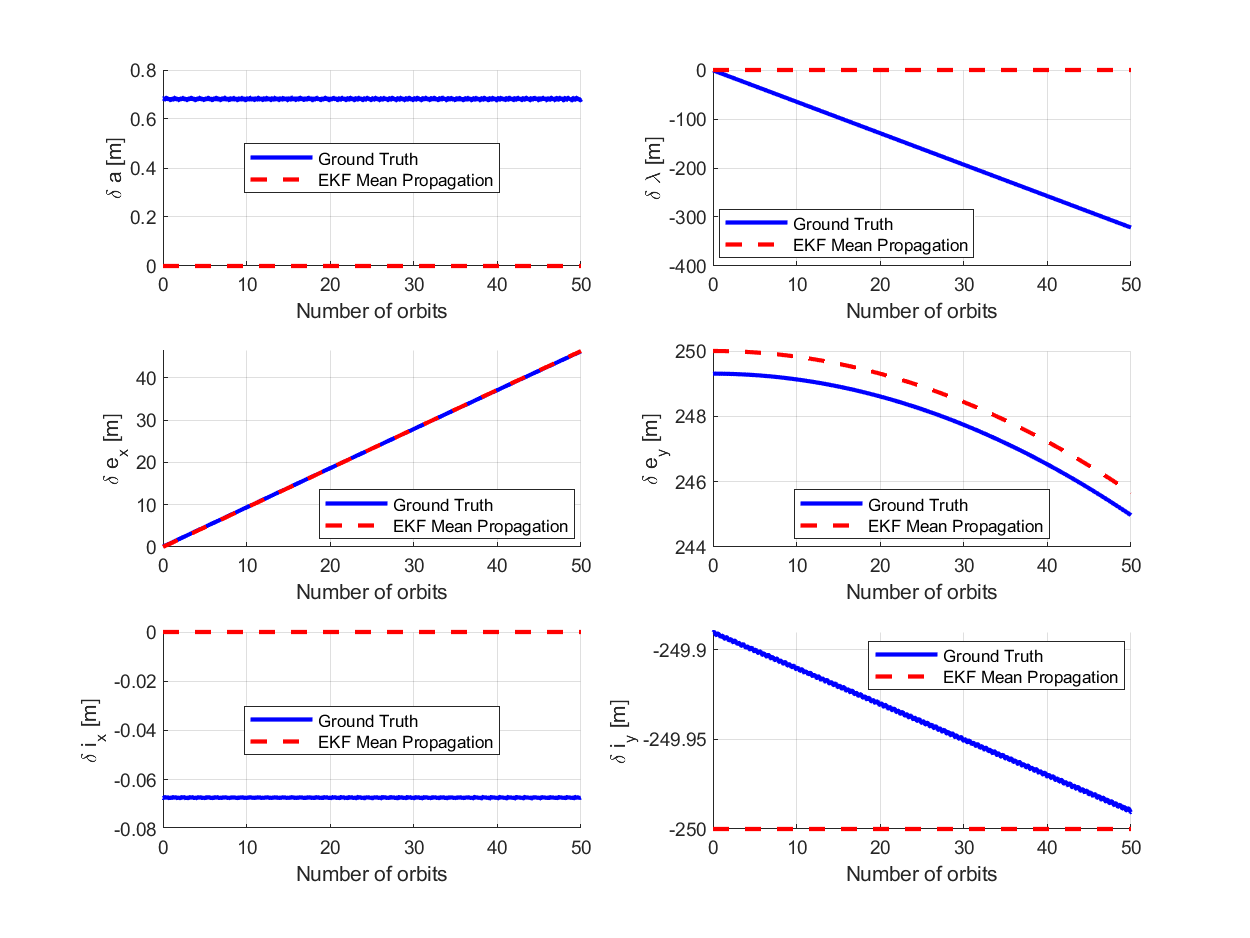
\includegraphics[width=0.75\linewidth]{sim/figures/PS7/ROE_over_time_SV3_comparison.png}
    \caption{ROE over time comparison for SV3}
    \label{fig:ROE_nonlinear_compare}
\end{figure}

The EKF Mean Propagation method aligns well with the ground truth for a propagation with no control inputs, showcasing J2 effects on $\delta e_x$ and $e_y$. In fact, it exhibits better behavior than the ground truth, since it has zero $\delta a$ and $\delta i_x$, which also means there is no $\delta \lambda$ or $\delta i_y$ drift from J2. The ground truth exhibits these drifts because of numerical error in the conversion from osculating to mean quantities that leads to nonzero $\delta a$ and $\delta i_x$, and an initial offset in $\delta e_x$. As such, the EKF Mean Propagation method is verified to be accurate. The ground truth propagation should be improved to remove the unexpected behavior it exhibits. 

\subsubsection{Linearized Dynamics Model for Covariance Update}
The dynamics models are linearized and then applied to the covariance update in the EKF.  

For the chief absolute orbit elements, the J2-induced secular drift rates with Keplerian motion added are:

\begin{align}
\frac{d e_x}{d t} &= -\frac{3}{4} n J_2 \left( \frac{R_E}{a \left( 1 - (e_x^2 + e_y^2) \right)} \right)^2 e_y (5 \cos^2 i - 1) \\
\frac{d e_y}{d t} &= \phantom{-}\frac{3}{4} n J_2 \left( \frac{R_E}{a \left( 1 - (e_x^2 + e_y^2) \right)} \right)^2 e_x (5 \cos^2 i - 1) \\
\frac{d \Omega}{d t} &= -\frac{3}{2} n J_2 \left( \frac{R_E}{a \left( 1 - (e_x^2 + e_y^2) \right)} \right)^2 \cos i  \\
\frac{d u}{d t} &= n + \frac{3}{4} n J_2 \left( \frac{R_E}{a \left( 1 - (e_x^2 + e_y^2) \right)} \right)^2 \left[ \sqrt{1 - (e_x^2 + e_y^2)} (3 \cos^2 i - 1) + (5 \cos^2 i - 1) \right] 
\end{align}

To get the STM, we now compute the Jacobian matrix \( \mathbf{A} = \partial \dot{\boldsymbol{\alpha}} / \partial \boldsymbol{\alpha} \) using first-order partials.

Let \( e^2 = e_x^2 + e_y^2 \), \( \eta = \sqrt{1 - e^2} \), and

\[
K = \frac{3}{4} n J_2 \left( \frac{R_E}{a(1 - e^2)} \right)^2
\]

Derivatives of \( \dot{e}_x \):
\[
\frac{\partial}{\partial e_y} \left( \frac{d e_x}{dt} \right) = -K (5 \cos^2 i - 1), \quad
\frac{\partial}{\partial i} \left( \frac{d e_x}{dt} \right) = -10 K e_y \cos i \sin i
\]

Derivatives of \( \dot{e}_y \):
\[
\frac{\partial}{\partial e_x} \left( \frac{d e_y}{dt} \right) = K (5 \cos^2 i - 1), \quad
\frac{\partial}{\partial i} \left( \frac{d e_y}{dt} \right) = 10 K e_x \cos i \sin i
\]

Derivative of \( \dot{\Omega} \):
\[
\frac{\partial}{\partial i} \left( \frac{d \Omega}{dt} \right) = 2K \sin i
\]

Derivatives of \( \dot{u} \):

\[
\frac{d u}{dt} = n + K \left[ \eta (3 \cos^2 i - 1) + (5 \cos^2 i - 1) \right]
\]

Partial w.r.t. \( e_x \):

\[
\frac{\partial \eta}{\partial e_x} = \frac{-e_x}{\eta}, \quad
\frac{\partial}{\partial e_x} \left( \frac{du}{dt} \right) = -K (3 \cos^2 i - 1) \cdot \frac{e_x}{\eta}
\]

Partial w.r.t. \( e_y \):

\[
\frac{\partial}{\partial e_y} \left( \frac{du}{dt} \right) = -K (3 \cos^2 i - 1) \cdot \frac{e_y}{\eta}
\]

Partial w.r.t. \( i \):

\[
\frac{\partial}{\partial i} \left( \frac{du}{dt} \right)
= K \cdot \frac{d}{di} \left[ \eta (3 \cos^2 i - 1) + (5 \cos^2 i - 1) \right]
= -6 K \cos i \sin i \left( \eta + \tfrac{5}{3} \right)
\]

Finally, putting all the partials together:

\[
\mathbf{A} =
\begin{bmatrix}
0 & 0 & 0 & 0 & 0 & 0 \\
0 & 0 & -K(5\cos^2 i - 1) & -10 K e_y \cos i \sin i & 0 & 0 \\
0 & K(5\cos^2 i - 1) & 0 & 10 K e_x \cos i \sin i & 0 & 0 \\
0 & 0 & 0 & 0 & 0 & 0 \\
0 & 0 & 0 & 2K \sin i & 0 & 0 \\
0 & -K(3 \cos^2 i - 1) \frac{e_x}{\eta} &
    -K(3 \cos^2 i - 1) \frac{e_y}{\eta} &
    -6K \cos i \sin i \left( \eta + \tfrac{5}{3} \right) & 0 & 0
\end{bmatrix}
\]

Then, the linearized STM for the absolute chief orbit elements is:

\[
\Phi(t, t_0) \approx \mathbf{I} + \mathbf{A} \, \Delta t
\]

For the relative orbit elements, the STM is given by \ref{eq:stm_matrix}. Together, these two STMs will be used to update covariance in the EKF. The control input matrix is given by Equation \ref{eq:control_input_matrix} is only relevant for the relative deputy states since the chief is not under control. Additionally, it is not dependent on the relative orbit elements state so it will not appear in the linearized covariance update equation. 

\subsubsection{On-board Sensors and Measurements}

Each of the deputies (SV2 and SV3) is equipped with the following sensors, which also give the raw measurements mentioned below:
\begin{itemize}
    \item \textbf{High-gain antennas:} Communication between the satellite and the ground is vital for higher accuracy measurements and an initialization of the orbital elements of our chief and deputy satellites. This can also enable us to get good measurements of the chief's orbital elements, which could be treated as true values when estimating the deputy satellites' positions.
    \item \textbf{Vision-based sensors + range sensor:} These provide relative bearing angle measurements for SV2 and SV3 relative to SV1. We assume that the sensors on SV2 and SV3 are always pointed at SV1. For close-range measurements required during SV3's docking phase, the vision-based sensors can also provide feature-rich images that may be used for more accurate position estimation. An additional range sensor is also used along with the vision sensor, to solve the range-ambiguity of purely perception-based navigation.
    \item \textbf{GNSS antennas:} These provide GNSS measurements such as pseudoranges. For simplicity, we stick with the single-difference GNSS pseudoranges. The single-difference DGNSS is enabled by inter-satellite links. Although, in the future, we will consider combining the pseudo-range measurements get to apply double-difference GNSS methods.
\end{itemize}

These raw measurements can be converted into simpler pseudo-measurements based on standard operations for each of the sensors. 
\begin{itemize}
    \item The relative bearing angle measurements of the vision-based sensor, $\alpha$ and $\epsilon$, along with the range measurement from a range sensor, can be converted into relative position vector measurements in the rectilinear frame $\boldsymbol{x}^\mathcal{R}$ \cite{sullivan2020nonlinear}. For this project, we make the simplifcation that the vision-based sensor gives us the pseudo-measurement of the relative position vector of the deputy in the chief's RTN frame.
    \item The psuedorange measurements acquired from the GNSS signals can be converted into absolute position measurements for the deputy satellites. For this project, we make the simplifcation that the GNSS sensors give us the psuedo-measurement of the absolute positions of the deputies in the ECI frame.
\end{itemize}
These pseudo-measurements are compiled into a measurement vector $y_{SV}$, for each spacecraft. For SV2, this is given by

\begin{align}
    y_{SV2} = \begin{bmatrix}
        \boldsymbol{r_{SV2}}^{RTN}\\
        \boldsymbol{x_{SV2}}^{ECI}
    \end{bmatrix}_{6\times 1}
\end{align}

A similar measurement vector $y_{SV3}$ is built for SV3. The combined full measurement vector, for both spacecraft together, is given by

\begin{align}
    y &= \begin{bmatrix}
        y_{SV2} \\
        y_{SV3}
    \end{bmatrix} \\
    &= \begin{bmatrix}
        \boldsymbol{r_{SV2}}^{RTN}\\
        \boldsymbol{r_{SV2}}^{ECI} \\
        \boldsymbol{r_{SV3}}^{RTN} \\
        \boldsymbol{r_{SV3}}^{ECI} \\
    \end{bmatrix}_{12\times 1}
\end{align}

An important note here is that although the chief's orbital elements are part of the state we are estimating, since the chief (SV1/Target) is not under active control and is a rogue spacecraft that we want to dock with, we do not receive any measurements specific to SV1. It is imperative, however, for us to have an estimate of SV1's motion to make sense of the absolute and relative measurements of SV2 and SV3.

For the purposes of this project, these measurements will just be noisy versions of the true states, with some added Gaussian noise. As such, no unit testing is required at this step.

\subsubsection{Measurement Model}
The measurement model relates the pseudo-measurements in $y$ from the vision-based sensors and the GNSS antennas to the state of the spacecrafts $x$, by some non-linear function $g(\cdot)$, i.e.
\begin{align}
    y_{SV2} &= g_{SV2}(\alpha_{1}, \delta \alpha _{2}) \\
    y_{SV3} &= g_{SV3}(\alpha_{1}, \delta \alpha _{2}) \\
    y &= g(x)
\end{align}

Here, $g(x):\mathbb{R}^{18} \rightarrow \mathbb{R}^{12}$ is a simple concatenation of each $g_{SV2}(\cdot)$ and $g_{SV3}(\cdot)$. For the selected pseudo-measurements, the measurement model we have converts our state-space representation that includes the chief's orbital elements and the deputy spacecraft's relative orbital elements into the pseudo-measurements of relative and absolute position vectors.

The conversion from relative orbital element to relative position vectors can be done in a non-linear fashion with higher fidelity by intermediately converting to absolute orbital elements, to ECI, and then to RTN. However, as shown in Chapter 2 of \cite{damicothesis}, for near-circular orbits we can find a linear mapping between the quasi-nonsingular relative orbital elements and position and velocity in the RTN frame (by relating the relative orbital elements to the integration constants in the Hill-Clohessy-Wiltshire equations). This is given by
\begin{align}
\boldsymbol{r}^{RTN} &\approx a_1
\begin{bmatrix}
1 & 0 & -\cos u_1 & -\sin u_1 & 0 & 0 \\
0 & 1 & 2\sin u_1 & -2\cos u_1 & 0 & 0 \\
0 & 0 & 0 & 0 & \sin u_1 & -\cos u_1 \\
\end{bmatrix}
\delta \boldsymbol{\alpha} \\
\boldsymbol{r}^{RTN} &\approx 
\mathcal{J}
a_1\delta \boldsymbol{\alpha} \\ \label{eq:J_linear_mapping}
\end{align}
where $u$ is the mean argument of latitude of the chief spacecraft. We use $\mathcal{J}_{3\times 6}$ to represent this transformation matrix. This is linear with respect to the deputy, but non-linear with respect to the chief's state.

The conversion from relative orbital elements to absolute position vectors can be done by converting to approximate RTN values as before, and then performing a rotation from relative RTN positions to ECI positions. The chief's ECI state is required here, which can also be converted from the chief's orbital elements.
\begin{align}
    \boldsymbol{r}^{ECI} = Q^\top_{eci2rtn} \boldsymbol{r}^{RTN} + \boldsymbol{r}_{SV1}^{ECI}
\end{align}
where $Q^\top_{eci2rtn}$ is defined using $\boldsymbol{r}_{SV1}^{ECI}$, as described in Equation \ref{eq:v_rtn_rel}. The calculation of $\boldsymbol{r}_{SV1}^{ECI}$ is itself a non-linear function of the chief's orbital elements, which is described in detail in Section \ref{sec:initial_ECI}. We can call this function $f_{oe2eci}(\cdot)$
\begin{align}
    \boldsymbol{r}_{SV1}^{ECI} = f_{oe2eci}(\boldsymbol{\alpha}_1)
\end{align}
With all these elements, we can now represent the measurement model and the relation between the state defined in Section \ref{sec:nav_state_rep} to our measurement vector.
\begin{align}
    y = &g(x) \\
    &g(x) = \begin{bmatrix}
        \mathcal{J}
a_1\delta \boldsymbol{\alpha}_2 \\
            Q^\top_{eci2rtn} \mathcal{J}
a_1\delta \boldsymbol{\alpha}_2 + f_{oe2eci}(\boldsymbol{\alpha}_1) \\
        \mathcal{J}
a_1\delta \boldsymbol{\alpha}_3 \\
            Q^\top_{eci2rtn} \mathcal{J}
a_1\delta \boldsymbol{\alpha}_3 + f_{oe2eci}(\boldsymbol{\alpha}_1) \\
    \end{bmatrix}_{12\times 1}
\end{align}

Since we are making some linear approximations in our measurement model, we plan on setting up some unit test cases to make sure this measurement model tracks. The unit test will verify that the measurement model aligns to some error tolerance (larger than the expected added noise) with the true measurements. If the residual between the measurements and the measurement model increases in any of the unit tests, then there is a case where the measurement model breaks down. The unit tests will help identify what these cases are, and where the measurement model might need improvements.

\subsubsection{Sensitivity Matrix}

The sensitivity matrix $C_t$ is formed by taking the Jacobian of the nonlinear function $g(x)$ with the current state value $x_t$. This gives us the linearized relation between the state vector $x_t$ and the measurement vector $y_t$.
\begin{align}
    y_t = C_tx_t\\
    C_t = \left . \frac{\partial g}{\partial x} \right|_{x = \bar{x}_t}
\end{align}

Taking the Jacobian, we get a matrix of dimensions $12 \times 18$. $C_t$ will be of the form
\begin{align}
    C_t = \left.\begin{bmatrix}
        \dfrac{\partial \mathcal{J}a_1 \delta \boldsymbol{\alpha}_2}{\partial \boldsymbol{\alpha}_1}  & \mathcal{J}a_1 & 0_{3\times6} \\
        \dfrac{Q^\top_{eci2rtn} \mathcal{J}
a_1\delta \boldsymbol{\alpha}_2 + f_{oe2eci}(\boldsymbol{\alpha}_1)}{\partial \boldsymbol{\alpha}_1} & Q^\top_{eci2rtn} \mathcal{J}
a_1 & 0_{3\times6} \\
        \dfrac{\partial \mathcal{J}a_1 \delta \boldsymbol{\alpha}_3}{\partial \boldsymbol{\alpha}_1}  & 0_{3\times6}  & \mathcal{J}a_1 \\
        \dfrac{Q^\top_{eci2rtn} \mathcal{J}
a_1\delta \boldsymbol{\alpha}_3 + f_{oe2eci}(\boldsymbol{\alpha}_1)}{\partial \boldsymbol{\alpha}_1} & 0_{3\times6} & Q^\top_{eci2rtn} \mathcal{J}
a_1\\
    \end{bmatrix} \right|_{x = \bar{x}_t}
\end{align}
The Jacobian is evaluated with $\bar{x}_t$, i.e. the value of the state at time $t$. This makes $C_t$ time-varying. In an Extended Kalman Filter, this sensitivity matrix $C_t$ is used to find the Kalman gain and thus update the state covariance estimate.

The inclusion of SV1's position in the state greatly complicates the calculation of the sensitivity matrix $C$. If this becomes restrictive when implementing the Kalman filter, then we may consider assuming perfect state knowledge of SV1, and only estimating the states of the deputies. 

It is critical that this formulation of the sensitivity matrix remain observable. Therefore, the unit tests here will check the condition number of the observability matrix over time for different short simulations, to ensure that the system is observable and the covariance of the state can be estimated.






